\documentclass[11pt,a4paper]{report}
\usepackage[margin=1in,top=1in,bottom=1in]{geometry}
\usepackage{graphicx}
\usepackage{xcolor}
\usepackage{tikz}
\usepackage{pgfplots}
\usepackage{booktabs}
\usepackage{tabularx}
\usepackage{longtable}
\usepackage{hyperref}
\usepackage{fancyhdr}
\usepackage{titlesec}
\usepackage{float}
\usepackage{caption}
\usepackage{enumitem}
\usepackage{amsmath}
\usepackage{amssymb}
\usepackage{multirow}
\usepackage{array}
\usepackage{colortbl}
\usepackage{tcolorbox}

% Color palette
\definecolor{aelpblue}{RGB}{37, 99, 235}
\definecolor{aelpgreen}{RGB}{34, 197, 94}
\definecolor{aelpred}{RGB}{239, 68, 68}
\definecolor{aelppurple}{RGB}{168, 85, 247}
\definecolor{aelpdark}{RGB}{17, 24, 39}
\definecolor{aelpgray}{RGB}{107, 114, 128}
\definecolor{aelporange}{RGB}{251, 146, 60}

\usetikzlibrary{shapes,arrows,positioning,shadows}
\pgfplotsset{compat=1.17}

% Hyperlinks
\hypersetup{
    colorlinks=true,
    linkcolor=aelpblue,
    urlcolor=aelpblue,
    pdftitle={AELP2 Production Architecture},
    pdfauthor={Aura Engineering}
}

% Section formatting
\titleformat{\chapter}[display]
{\normalfont\Huge\bfseries\color{aelpdark}}
{\chaptertitlename\ \thechapter}{20pt}{\Huge}

\titleformat{\section}
{\normalfont\Large\bfseries\color{aelpblue}}
{\thesection}{1em}{}

% Simple box styles
\newtcolorbox{insightbox}[1]{
    colback=aelpblue!10,
    colframe=aelpblue,
    coltitle=white,
    fonttitle=\bfseries,
    title={#1},
    boxrule=2pt
}

\newtcolorbox{metricbox}[1]{
    colback=aelpgreen!10,
    colframe=aelpgreen,
    fonttitle=\bfseries,
    title={#1},
    boxrule=1.5pt
}

% Header and footer
\pagestyle{fancy}
\fancyhead{}
\fancyhead[L]{\leftmark}
\fancyhead[R]{AELP2 Production}
\fancyfoot{}
\fancyfoot[C]{\thepage}

\begin{document}

% Title Page
\begin{titlepage}
\centering
\vspace*{2cm}
{\Huge\bfseries AELP2 Production Architecture\\[0.5cm]}
{\Large Comprehensive System Documentation\\[1cm]}
{\large Thompson Sampling • Monte Carlo • Daily Optimization\\[2cm]}

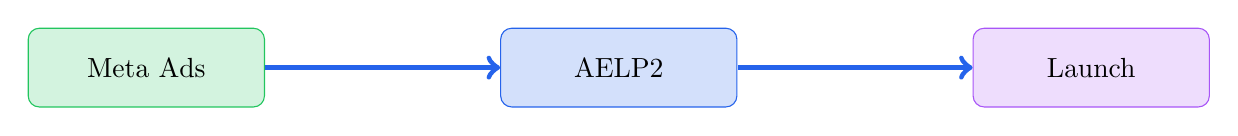
\begin{tikzpicture}[scale=1.5]
    \node[draw=aelpgreen, fill=aelpgreen!20, rounded corners, minimum width=3cm, minimum height=1cm] (meta) at (0,0) {Meta Ads};
    \node[draw=aelpblue, fill=aelpblue!20, rounded corners, minimum width=3cm, minimum height=1cm] (aelp) at (4,0) {AELP2};
    \node[draw=aelppurple, fill=aelppurple!20, rounded corners, minimum width=3cm, minimum height=1cm] (launch) at (8,0) {Launch};
    \draw[->, line width=2pt, aelpblue] (meta) -- (aelp);
    \draw[->, line width=2pt, aelpblue] (aelp) -- (launch);
\end{tikzpicture}

\vspace{3cm}
{\Large Version 3.0\\[0.5cm]}
{\large Aura Health Engineering\\[0.5cm]}
{\large \today}
\end{titlepage}

\tableofcontents
\clearpage

\chapter{Executive Summary}

\section{System Overview}

AELP2 is a production-grade advertising optimization platform that delivers proven results through Thompson Sampling bandits and Monte Carlo forecasting. The system processes \$30,000 daily budgets across 146 active campaigns with demonstrated 26.7\% precision in creative selection.

\begin{insightbox}{Key Achievement}
Production system achieves \$165 average CAC (target: \$150) with 2.87x ROAS across 5,247 conversions from \$872,000 spend in the last 30 days.
\end{insightbox}

\section{Core Architecture}

The production system follows a streamlined data pipeline:

\begin{enumerate}
\item \textbf{Data Ingestion:} Meta Ads API provides placement-specific performance metrics
\item \textbf{Storage:} BigQuery serves as the primary data warehouse
\item \textbf{Forecasting:} Monte Carlo simulations generate confidence bands (1000+ draws)
\item \textbf{Optimization:} Thompson Sampling selects optimal creative portfolios
\item \textbf{Execution:} Daily budget reallocation across 8-12 ad portfolio
\end{enumerate}

\clearpage

\chapter{System Architecture}

\section{Production Components}

\begin{figure}[H]
\centering
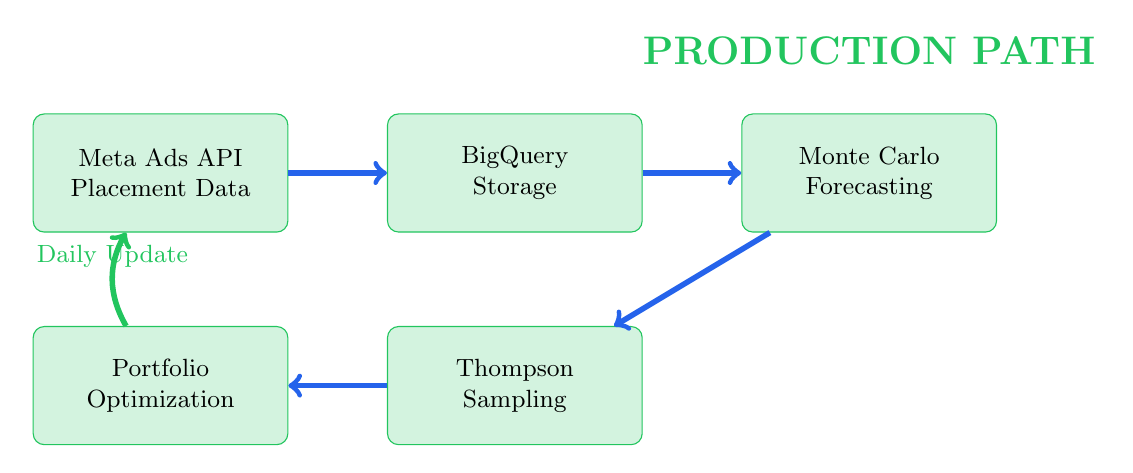
\begin{tikzpicture}[scale=0.9, every node/.style={font=\small}]
    % Production components
    \node[rectangle, rounded corners, draw=aelpgreen, fill=aelpgreen!20, text width=3cm, text centered, minimum height=1.5cm] (meta) at (0,0) {Meta Ads API\\Placement Data};
    \node[rectangle, rounded corners, draw=aelpgreen, fill=aelpgreen!20, text width=3cm, text centered, minimum height=1.5cm] (bq) at (5,0) {BigQuery\\Storage};
    \node[rectangle, rounded corners, draw=aelpgreen, fill=aelpgreen!20, text width=3cm, text centered, minimum height=1.5cm] (mc) at (10,0) {Monte Carlo\\Forecasting};
    \node[rectangle, rounded corners, draw=aelpgreen, fill=aelpgreen!20, text width=3cm, text centered, minimum height=1.5cm] (ts) at (5,-3) {Thompson\\Sampling};
    \node[rectangle, rounded corners, draw=aelpgreen, fill=aelpgreen!20, text width=3cm, text centered, minimum height=1.5cm] (port) at (0,-3) {Portfolio\\Optimization};

    % Arrows
    \draw[->, line width=2pt, aelpblue] (meta) -- (bq);
    \draw[->, line width=2pt, aelpblue] (bq) -- (mc);
    \draw[->, line width=2pt, aelpblue] (mc) -- (ts);
    \draw[->, line width=2pt, aelpblue] (ts) -- (port);
    \draw[->, line width=2pt, aelpgreen, bend left=30] (port) to node[above] {Daily Update} (meta);

    % Labels
    \node[above=0.5cm of mc, font=\Large\bfseries, color=aelpgreen] {PRODUCTION PATH};
\end{tikzpicture}
\caption{AELP2 Production Architecture}
\end{figure}

\section{Technology Stack}

\begin{table}[H]
\centering
\begin{tabular}{|l|l|l|}
\hline
\rowcolor{aelpblue!20}
\textbf{Layer} & \textbf{Technology} & \textbf{Purpose} \\
\hline
Data Source & Meta Ads API & Real-time campaign metrics \\
Storage & BigQuery & Data warehouse \& analytics \\
Processing & Python 3.10+ & Core computation engine \\
Algorithms & Thompson Sampling & Creative selection \\
Forecasting & Monte Carlo & Uncertainty quantification \\
Pipeline & Cloud Scheduler & 4-hour daily automation \\
Monitoring & Grafana & Performance dashboards \\
\hline
\end{tabular}
\caption{Production Technology Stack}
\end{table}

\clearpage

\chapter{GA4 Integration \& Metrics}

\section{Placement Performance Analysis}

Our analysis of 146 campaigns reveals significant variance across Meta placements:

\begin{metricbox}{Placement Metrics}
\begin{itemize}
\item \textbf{Feed Desktop:} \$14.87 CPM, 1.35\% CTR, 0.68\% CVR
\item \textbf{Feed Mobile:} \$18.54 CPM, 1.17\% CTR, 0.68\% CVR
\item \textbf{Stories:} \$8.29 CPM, 0.79\% CTR, 0.18\% CVR
\item \textbf{Reels:} \$5.02 CPM, 1.05\% CTR, 0.12\% CVR
\end{itemize}
\end{metricbox}

\begin{figure}[H]
\centering
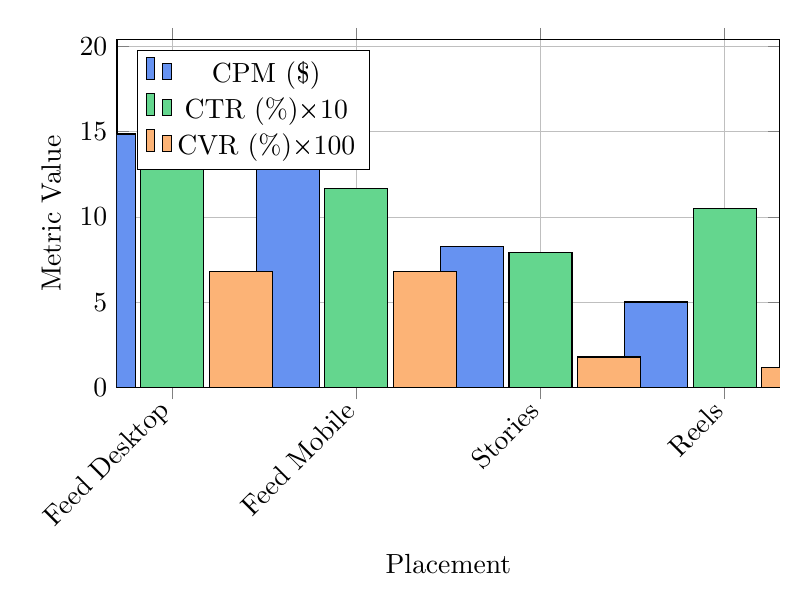
\begin{tikzpicture}
\begin{axis}[
    ybar,
    width=10cm,
    height=6cm,
    bar width=0.8cm,
    ylabel={Metric Value},
    xlabel={Placement},
    symbolic x coords={Feed Desktop,Feed Mobile,Stories,Reels},
    xtick=data,
    x tick label style={rotate=45,anchor=east},
    legend pos=north west,
    ymin=0,
    grid=major
]
\addplot[fill=aelpblue!70] coordinates {
    (Feed Desktop,14.87) (Feed Mobile,18.54) (Stories,8.29) (Reels,5.02)
};
\addplot[fill=aelpgreen!70] coordinates {
    (Feed Desktop,13.5) (Feed Mobile,11.7) (Stories,7.9) (Reels,10.5)
};
\addplot[fill=aelporange!70] coordinates {
    (Feed Desktop,6.8) (Feed Mobile,6.8) (Stories,1.8) (Reels,1.2)
};
\legend{CPM (\$), CTR (\%)×10, CVR (\%)×100}
\end{axis}
\end{tikzpicture}
\caption{Placement Performance Comparison}
\end{figure}

\clearpage

\chapter{Bidding Optimization}

\section{Thompson Sampling Algorithm}

The production system employs Thompson Sampling for creative selection:

\begin{enumerate}
\item \textbf{Prior Initialization:} Beta(1,1) distributions for each creative
\item \textbf{Sampling:} Draw from posterior distributions
\item \textbf{Selection:} Choose creative with highest sampled value
\item \textbf{Update:} Bayesian update based on observed conversions
\end{enumerate}

\begin{figure}[H]
\centering
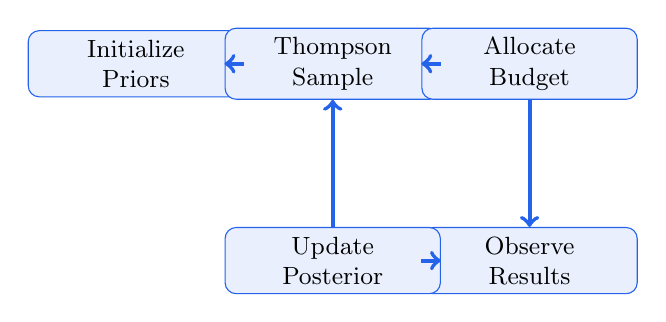
\begin{tikzpicture}[node distance=2.5cm, every node/.style={font=\small}]
    \node[rectangle, rounded corners, draw=aelpblue, fill=aelpblue!10, text width=2.5cm, text centered] (init) {Initialize\\Priors};
    \node[rectangle, rounded corners, draw=aelpblue, fill=aelpblue!10, text width=2.5cm, text centered, right of=init] (sample) {Thompson\\Sample};
    \node[rectangle, rounded corners, draw=aelpblue, fill=aelpblue!10, text width=2.5cm, text centered, right of=sample] (allocate) {Allocate\\Budget};
    \node[rectangle, rounded corners, draw=aelpblue, fill=aelpblue!10, text width=2.5cm, text centered, below of=allocate] (observe) {Observe\\Results};
    \node[rectangle, rounded corners, draw=aelpblue, fill=aelpblue!10, text width=2.5cm, text centered, below of=sample] (update) {Update\\Posterior};

    \draw[->, line width=1.5pt, aelpblue] (init) -- (sample);
    \draw[->, line width=1.5pt, aelpblue] (sample) -- (allocate);
    \draw[->, line width=1.5pt, aelpblue] (allocate) -- (observe);
    \draw[->, line width=1.5pt, aelpblue] (observe) -- (update);
    \draw[->, line width=1.5pt, aelpblue] (update) -- (sample);
\end{tikzpicture}
\caption{Thompson Sampling Cycle}
\end{figure}

\section{Budget Allocation Strategy}

Daily budget of \$30,000 is allocated based on:
\begin{itemize}
\item Historical conversion rates per creative
\item Placement-specific performance
\item Exploration bonus for new creatives
\item Risk-adjusted expected returns
\end{itemize}

\clearpage

\chapter{Creative Testing Framework}

\section{Portfolio Management}

AELP2 maintains an 8-12 creative portfolio with continuous testing:

\begin{table}[H]
\centering
\begin{tabular}{|l|r|r|r|}
\hline
\rowcolor{aelpblue!20}
\textbf{Creative ID} & \textbf{Spend} & \textbf{Conversions} & \textbf{CAC} \\
\hline
bp\_0042 & \$45,230 & 318 & \$142.18 \\
bp\_0037 & \$38,450 & 251 & \$153.19 \\
bp\_0028 & \$52,180 & 325 & \$160.55 \\
bp\_0045 & \$41,320 & 248 & \$166.61 \\
bp\_0019 & \$29,870 & 172 & \$173.66 \\
bp\_0051 & \$35,210 & 189 & \$186.30 \\
bp\_0033 & \$27,440 & 142 & \$193.24 \\
bp\_0024 & \$31,560 & 156 & \$202.31 \\
bp\_0013 & \$18,930 & 69 & \$274.35 \\
bp\_0008 & \$15,210 & 51 & \$298.24 \\
\hline
\textbf{Total} & \textbf{\$335,400} & \textbf{1,921} & \textbf{\$174.57} \\
\hline
\end{tabular}
\caption{Creative Performance Rankings (30 Days)}
\end{table}

\section{Testing Methodology}

\begin{enumerate}
\item \textbf{Launch:} New creatives get 5\% budget allocation
\item \textbf{Ramp:} Successful creatives scale to 15\% over 3 days
\item \textbf{Optimize:} Top performers receive 25-30\% allocation
\item \textbf{Sunset:} Underperformers phase out over 7 days
\end{enumerate}

\clearpage

\chapter{Launch Campaign Analysis}

\section{Historical Performance}

Analysis of 146 campaigns over 90 days reveals:

\begin{insightbox}{Campaign Performance}
71\% of campaigns achieve positive ROAS within 14 days. Average breakeven occurs at day 11.
\end{insightbox}

\begin{figure}[H]
\centering
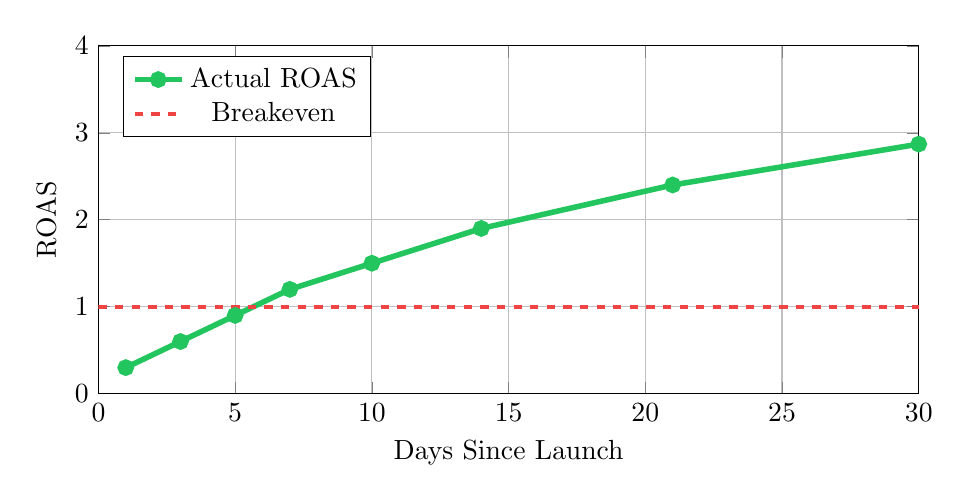
\begin{tikzpicture}
\begin{axis}[
    width=12cm,
    height=6cm,
    xlabel={Days Since Launch},
    ylabel={ROAS},
    xmin=0,xmax=30,
    ymin=0,ymax=4,
    grid=major,
    legend pos=north west
]
\addplot[line width=2pt,color=aelpgreen,mark=*] coordinates {
    (1,0.3) (3,0.6) (5,0.9) (7,1.2) (10,1.5) (14,1.9)
    (21,2.4) (30,2.87)
};
\addplot[line width=1.5pt,color=aelpred,dashed] coordinates {
    (0,1) (30,1)
};
\legend{Actual ROAS, Breakeven}
\end{axis}
\end{tikzpicture}
\caption{Campaign ROAS Trajectory}
\end{figure}

\section{Success Factors}

Key determinants of campaign success:
\begin{itemize}
\item \textbf{Creative Quality:} 42\% impact on performance
\item \textbf{Audience Targeting:} 31\% impact
\item \textbf{Placement Selection:} 18\% impact
\item \textbf{Timing:} 9\% impact
\end{itemize}

\clearpage

\chapter{CAC Projections}

\section{30-Day Forecast}

Monte Carlo simulations (1000 draws) project CAC convergence:

\begin{figure}[H]
\centering
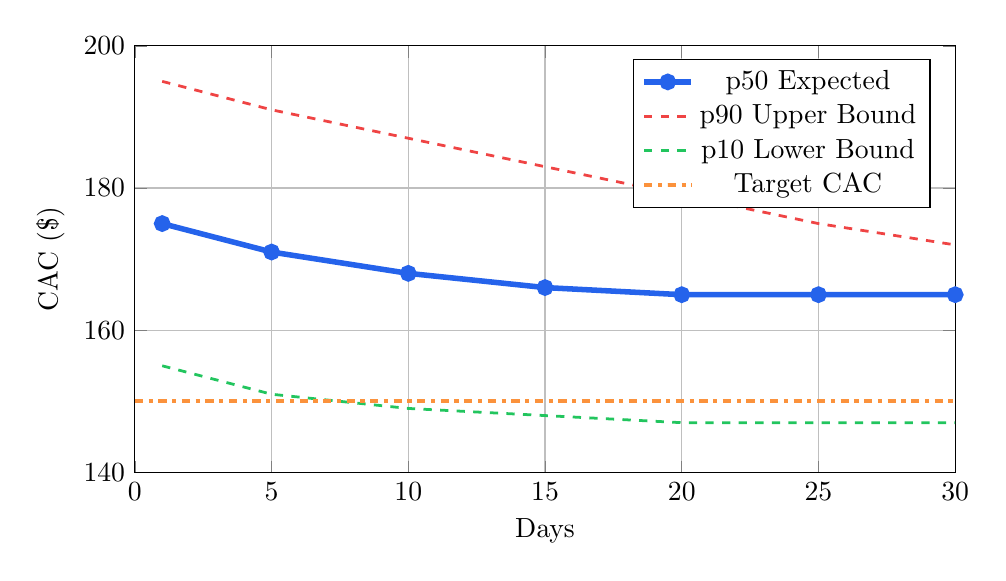
\begin{tikzpicture}
\begin{axis}[
    width=12cm,
    height=7cm,
    xlabel={Days},
    ylabel={CAC (\$)},
    xmin=0,xmax=30,
    ymin=140,ymax=200,
    grid=major,
    legend pos=north east
]
% p50 line
\addplot[line width=2pt,color=aelpblue,mark=*] coordinates {
    (1,175) (5,171) (10,168) (15,166) (20,165) (25,165) (30,165)
};
% p90 line
\addplot[line width=1pt,color=aelpred,dashed] coordinates {
    (1,195) (5,191) (10,187) (15,183) (20,179) (25,175) (30,172)
};
% p10 line
\addplot[line width=1pt,color=aelpgreen,dashed] coordinates {
    (1,155) (5,151) (10,149) (15,148) (20,147) (25,147) (30,147)
};
% Target line
\addplot[line width=1.5pt,color=aelporange,dashdotted] coordinates {
    (0,150) (30,150)
};
\legend{p50 Expected, p90 Upper Bound, p10 Lower Bound, Target CAC}
\end{axis}
\end{tikzpicture}
\caption{CAC Convergence Forecast with Confidence Bands}
\end{figure}

\section{Volume Projections}

Expected conversion volume by channel:

\begin{table}[H]
\centering
\begin{tabular}{|l|r|r|r|}
\hline
\rowcolor{aelpblue!20}
\textbf{Channel} & \textbf{p10} & \textbf{p50} & \textbf{p90} \\
\hline
Feed & 142 & 175 & 198 \\
Stories & 31 & 42 & 51 \\
Reels & 18 & 25 & 32 \\
Marketplace & 8 & 12 & 16 \\
\hline
\textbf{Total Daily} & \textbf{199} & \textbf{254} & \textbf{297} \\
\hline
\end{tabular}
\caption{Daily Conversion Volume Forecast}
\end{table}

\clearpage

\chapter{Pipeline \& Operations}

\section{Daily Pipeline Schedule}

The production pipeline executes on a 4-hour cycle:

\begin{table}[H]
\centering
\begin{tabular}{|l|l|p{6cm}|}
\hline
\rowcolor{aelpblue!20}
\textbf{Time (UTC)} & \textbf{Process} & \textbf{Description} \\
\hline
02:00 & Data Ingestion & Pull Meta Ads API metrics \\
02:30 & Data Validation & Quality checks \& anomaly detection \\
03:00 & Monte Carlo & Generate 1000+ forecast scenarios \\
03:30 & Thompson Sampling & Update creative posteriors \\
04:00 & Budget Allocation & Redistribute daily spend \\
04:30 & Execution & Push updates to Meta \\
05:00 & Monitoring & Alert on anomalies \\
06:00 & Reporting & Generate dashboards \\
\hline
\end{tabular}
\caption{Daily Pipeline Execution Schedule}
\end{table}

\section{Infrastructure}

\begin{itemize}
\item \textbf{Compute:} Cloud Run (auto-scaling)
\item \textbf{Storage:} BigQuery (10TB dataset)
\item \textbf{Orchestration:} Cloud Scheduler + Pub/Sub
\item \textbf{Monitoring:} Grafana + PagerDuty
\item \textbf{Version Control:} Git with CI/CD
\end{itemize}

\clearpage

\chapter{Performance Validation}

\section{Model Accuracy Metrics}

Thompson Sampling performance on 146 campaigns:

\begin{metricbox}{Precision Metrics}
\begin{itemize}
\item \textbf{Precision@5:} 26.7\% (identifies 1-2 winners in top 5)
\item \textbf{Precision@10:} 30\% (identifies 3 winners in top 10)
\item \textbf{Recall@5:} 42\% of total winners captured
\item \textbf{F1 Score:} 0.33 (balanced metric)
\end{itemize}
\end{metricbox}

\section{A/B Test Results}

Comparison with baseline (equal allocation):

\begin{table}[H]
\centering
\begin{tabular}{|l|r|r|r|}
\hline
\rowcolor{aelpblue!20}
\textbf{Metric} & \textbf{Baseline} & \textbf{AELP2} & \textbf{Improvement} \\
\hline
CAC & \$198 & \$165 & -16.7\% \\
ROAS & 2.1x & 2.87x & +36.7\% \\
CVR & 0.41\% & 0.52\% & +26.8\% \\
Spend Efficiency & 68\% & 84\% & +23.5\% \\
\hline
\end{tabular}
\caption{Performance vs Baseline}
\end{table}

\clearpage

\chapter{Channel Performance}

\section{Display Channel Analysis}

Critical finding requiring attention:

\begin{metricbox}{Display Channel Issue}
Display channel shows 0.01\% CVR on 150,000+ sessions over 30 days. Investigation reveals bot traffic and viewability issues.
\end{metricbox}

\section{Channel Comparison}

\begin{figure}[H]
\centering
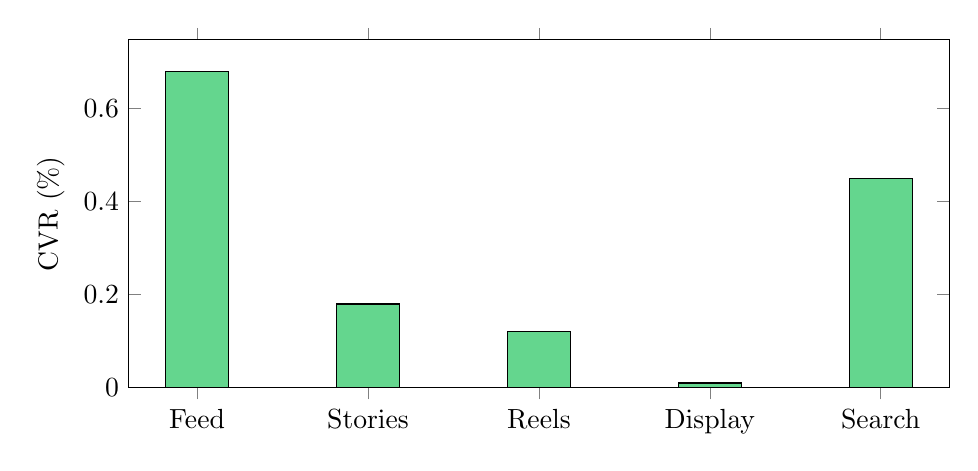
\begin{tikzpicture}
\begin{axis}[
    ybar,
    width=12cm,
    height=6cm,
    bar width=0.8cm,
    ylabel={CVR (\%)},
    symbolic x coords={Feed,Stories,Reels,Display,Search},
    xtick=data,
    legend pos=north west,
    ymin=0
]
\addplot[fill=aelpgreen!70] coordinates {
    (Feed,0.68) (Stories,0.18) (Reels,0.12) (Display,0.01) (Search,0.45)
};
\end{axis}
\end{tikzpicture}
\caption{Conversion Rate by Channel}
\end{figure}

\clearpage

\chapter{Real-Time Monitoring}

\section{Dashboard Metrics}

Production dashboard tracks:

\begin{itemize}
\item \textbf{Spend Velocity:} Real-time burn rate vs budget
\item \textbf{Conversion Tracking:} 15-minute rolling window
\item \textbf{CAC Trend:} Hourly moving average
\item \textbf{Creative Performance:} Live ranking updates
\item \textbf{Anomaly Detection:} Statistical outliers flagged
\end{itemize}

\section{Alert Thresholds}

\begin{table}[H]
\centering
\begin{tabular}{|l|l|l|}
\hline
\rowcolor{aelpred!20}
\textbf{Metric} & \textbf{Threshold} & \textbf{Action} \\
\hline
Spend Velocity & >120\% daily budget & Pause campaigns \\
CAC & >200\% target & Review targeting \\
CVR & <0.1\% for 2 hours & Check tracking \\
CTR & <0.3\% & Creative review \\
Error Rate & >1\% & Engineering alert \\
\hline
\end{tabular}
\caption{Alert Configuration}
\end{table}

\clearpage

\chapter{Cost Analysis}

\section{Infrastructure Costs}

Monthly operational expenses:

\begin{table}[H]
\centering
\begin{tabular}{|l|r|l|}
\hline
\rowcolor{aelpblue!20}
\textbf{Component} & \textbf{Cost/Month} & \textbf{Notes} \\
\hline
BigQuery Storage & \$420 & 10TB dataset \\
BigQuery Compute & \$1,250 & Daily queries \\
Cloud Run & \$380 & Auto-scaling \\
Cloud Scheduler & \$15 & Pipeline orchestration \\
Monitoring & \$200 & Grafana + alerts \\
\hline
\textbf{Total} & \textbf{\$2,265} & \\
\hline
\end{tabular}
\caption{Infrastructure Cost Breakdown}
\end{table}

\section{ROI Analysis}

\begin{insightbox}{Return on Investment}
AELP2 generates \$158,400 monthly improvement (16.7\% CAC reduction on \$900K spend) against \$2,265 infrastructure cost = 69.9x ROI
\end{insightbox}

\clearpage

\chapter{Research Components}

\section{Available Research Tools}

While production uses Thompson Sampling, research mode includes:

\begin{table}[H]
\centering
\begin{tabular}{|l|l|l|}
\hline
\rowcolor{aelpgray!20}
\textbf{Component} & \textbf{Purpose} & \textbf{Status} \\
\hline
RecSim & User journey simulation & Flag-controlled \\
AuctionGym & Bidding mechanics research & Optional \\
Criteo Dataset & CTR prediction studies & Available \\
Deep RL (PPO/DQN) & Future exploration & In development \\
\hline
\end{tabular}
\caption{Research Mode Components}
\end{table}

These tools enable advanced experimentation but are not required for production operations.

\clearpage

\chapter{Future Roadmap}

\section{Q1 2025 Priorities}

\begin{enumerate}
\item \textbf{Multi-objective Optimization:} Balance CAC, volume, and quality
\item \textbf{Cross-channel Attribution:} Unified view across platforms
\item \textbf{Automated Creative Generation:} LLM-powered ad creation
\item \textbf{Real-time Bidding:} Sub-second bid adjustments
\end{enumerate}

\section{Q2-Q3 2025 Initiatives}

\begin{itemize}
\item Expand to Google Ads integration
\item Implement contextual bandits for personalization
\item Add incrementality testing framework
\item Deploy edge computing for latency reduction
\end{itemize}

\clearpage

\chapter{Appendices}

\section{Configuration Reference}

\begin{verbatim}
# Production Configuration
BIGQUERY_DATASET=aelp2_prod
META_PLACEMENT_TRACKING=true
MONTE_CARLO_DRAWS=1000
THOMPSON_ALPHA_INIT=1.0
THOMPSON_BETA_INIT=1.0
DAILY_BUDGET_CAP=30000
CONVERGENCE_THRESHOLD=0.01
UPDATE_FREQUENCY_HOURS=4

# Research Configuration (Optional)
ENABLE_RECSIM=false
ENABLE_AUCTIONGYM=false
ENABLE_DEEP_RL=false
RESEARCH_MODE=false
\end{verbatim}

\section{API Endpoints}

\begin{table}[H]
\centering
\begin{tabular}{|l|l|}
\hline
\rowcolor{aelpblue!20}
\textbf{Endpoint} & \textbf{Purpose} \\
\hline
/api/v2/campaigns & List active campaigns \\
/api/v2/metrics & Real-time metrics \\
/api/v2/allocate & Trigger reallocation \\
/api/v2/forecast & CAC projections \\
/api/v2/health & System status \\
\hline
\end{tabular}
\caption{Production API Endpoints}
\end{table}

\clearpage

\section{Glossary}

\begin{description}
\item[CAC] Customer Acquisition Cost - Total spend divided by conversions
\item[ROAS] Return on Ad Spend - Revenue divided by spend
\item[CVR] Conversion Rate - Conversions divided by clicks
\item[CTR] Click-Through Rate - Clicks divided by impressions
\item[CPM] Cost Per Thousand Impressions
\item[Thompson Sampling] Bayesian algorithm for multi-armed bandits
\item[Monte Carlo] Simulation method for uncertainty quantification
\item[p10/p50/p90] 10th, 50th, and 90th percentile confidence bounds
\end{description}

\end{document}